\documentclass[uplatex]{jsarticle}

% パッケージ
\usepackage[dvipdfmx]{hyperref, graphicx}
\usepackage{pxjahyper}
\usepackage{siunitx} % SI単位
\usepackage{amssymb}
\usepackage{amsmath}
\usepackage{caption,subcaption}
\usepackage[top=20truemm,bottom=20truemm,left=25truemm,right=25truemm]{geometry}
\usepackage{here}
\usepackage{ascmac} % 枠付き文章


\hypersetup{
    colorlinks=false, % リンクに色をつけない設定
    bookmarks=true, % 以下ブックマークに関する設定
    bookmarksnumbered=true,
    pdfborder={0 0 0},
    bookmarkstype=toc,
}

\newcommand{\linedhref}[2]{\underline{\href{#1}{\emph{#2}}}}

% 接頭辞の設定
\renewcommand{\figurename}{Fig.}
\renewcommand{\tablename}{Table.}
\newcommand\figref[1]{{図~\ref{fig:#1}}}
\newcommand\tabref[1]{{表~\ref{tab:#1}}}
\newcommand\eref[1]{{式~({\boldmath \ref{eq:#1}})}}
\newcommand\secref[1]{{第~\ref{sec:#1}章}}
\newcommand\ssecref[1]{{~\ref{sec:#1}節}}
\def\abstractname{要旨}
\def\prepartname{第}
\def\postpartname{章}

% 自作関数
\newcommand{\divergence}{\mathrm{div}\,}  %ダイバージェンス
\newcommand{\grad}{\mathrm{grad}\,}  %グラディエント
\newcommand{\rot}{\mathrm{rot}\,}  %ローテーション
\def\vector#1{\mbox{\boldmath $#1$}}
\newcommand{\e}{\mathrm{e}} %自然対数
\newcommand{\pdiff}[3]{
    \if 1#1 \dfrac{\partial #2}{\partial #3}
    \else \dfrac{\partial^{#1} #2}{\partial #3^{#1}}\fi
}

% Captionの設定
% \captionwidth=0.8\textwidth
\captionsetup[figure]{font=small}
\captionsetup[table]{font=small} %small=9pt,footnotesize=8pt}
\abovecaptionskip=5pt
\belowcaptionskip=0pt
\title{\LaTeX のサンプルソース}
\author{a11-green}

\begin{document}
\maketitle
\tableofcontents

\newpage
\section{はじめに}
このミカンの大きさは1 \si{m}である\cite{Soseki1905}。

\section{基本文法}
\subsection{図}
図を張るためのソースはユーザスニペットとして登録している。1枚のみはる場合は次のようになる。
\begin{figure}[H]
	\centering
	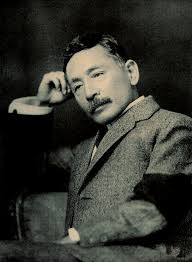
\includegraphics[width=0.5\textwidth]{figure/natsume_soseki.jpeg}
	\caption{夏目漱石の写真\cite{Soseki1905}。あああああああああああああああああああああああああああああああ}
	\label{fig:夏目漱石の写真}
\end{figure}


\subsection{数式}
連続の式は\eref{mass-conservation}のように表される。
式の参照について、式のラベル名にeq:をつけることで、erefコマンドによりeq:の後の文字列を指定することで式(・)として参照できるようにしている。
またよく使う偏微分はpdiffコマンドで簡単に記述できるようにしている。
詳しくはソースコードを参照されたい。
\begin{align}
	\pdiff{1}{u}{x} + \pdiff{1}{v}{y} + \pdiff{1}{w}{z} = 0
	\label{eq:mass-conservation}
\end{align}



\bibliography{ref}
\bibliographystyle{junsrt}

\end{document}